\documentclass[a4paper, 7pt, landscape]{scrartcl}
\usepackage[german]{babel}
\usepackage[utf8]{inputenc}
\usepackage{multicol}
\usepackage{geometry}
\usepackage{graphicx}
\usepackage{wrapfig}
\usepackage{enumitem}
\usepackage{fancyhdr}
\usepackage{index}
\usepackage{sectsty}
\usepackage{mwe}
\usepackage{comment}
\usepackage{lipsum}
\usepackage{titlesec}
\usepackage[dvipsnames]{xcolor}
\usepackage{amsmath}
\usepackage{amssymb}
\usepackage{listings}

%Define Math Commands:
\newcommand*{\field}[1]{\mathbb{#1}}%
\newcommand{\Mod}[1]{\ (\mathrm{mod}\ #1)}

%Image Folder:
\graphicspath{{../img/}}

%format
\geometry{top=0.4cm,left=0.5cm,right=0.5cm,bottom=0.4cm}
\setlist{topsep=0pt, leftmargin=5mm, nolistsep}

% Code Snippets

\definecolor{javared}{rgb}{0.6,0,0} % for strings

\lstset{
language=C,
basicstyle=\fontsize{7}{7} \ttfamily,
keywordstyle=\bfseries\color{RoyalBlue},
stringstyle=\color{javared},
commentstyle=\color{MidnightBlue},
morecomment=[s][\color{MidnightBlue}]{/**}{*/},
tabsize=2,
showspaces=false,
showstringspaces=false,
texcl = true,
rulecolor = \color{black},
breaklines = true,
aboveskip = 0em,
belowskip = 0em
}




% Define Section Format
\titleformat{name=\section}[block]
{\sffamily\normalsize}
{}
{0pt}
{\colorsection}
\titlespacing*{\section}{0pt}{0pt}{0pt}

\newcommand{\colorsection}[1]{%
\colorbox{MidnightBlue!40}{\parbox{0.98\linewidth}{\color{black}\thesection\ #1}}}


% Define Subsection Format
\titleformat{name=\subsection}[block]
{\sffamily\small}
{}
{0pt}
{\colorsubsection}
\titlespacing*{\subsection}{0pt}{0pt}{0pt}

\newcommand{\colorsubsection}[1]{%
\colorbox{YellowGreen!50}{\parbox{0.98\linewidth}{\color{black}\thesubsection\ #1}}}

% Define SubSubsection Format
\titleformat{name=\subsubsection}[block]
{\sffamily\small}
{}
{0pt}
{\colorsubsubsection}
\titlespacing*{\subsubsection}{0pt}{0pt}{0pt}

\newcommand{\colorsubsubsection}[1]{%
\colorbox{Goldenrod!50}{\parbox{0.98\linewidth}{\color{black}\thesubsubsection\ #1}}}

% -----------------------------------------------------------------------
\begin{document}
    %	\pagecolor{p}
    %	\color{t}
    \setlength{\columnseprule}{0.4pt}
    \footnotesize
    \begin{multicols*}{3}

        %! Author = Philipp Emmenegger
%! Date = 30/06/2021

\section{Introduction}
\textbf{Artificial Intelligence (AGI)}
\begin{itemize}
    \item broad concept
    \item different interpretations
    \item we do not have a definition of intelligence
    \item a hypothetical computer program that can perform intellectual tasks as well or better than a human
\end{itemize}
\vspace{10pt}
\textcolor{blue}{Examples of application (today)}
\begin{itemize}
    \item Personalization of news feeds
    \item Product searching and recommendation s on eCommerce platforms
    \item Voice-to-text
    \item Predictive maintenance
\end{itemize}
\vspace{10pt}
\textbf{Statistical machine learning}
\begin{itemize}
    \item Algorithms and applications where computer learn from data
\end{itemize}
\vspace{10pt}
\textbf{Turing Test}
\begin{itemize}
    \item Also called imitation game
    \item Tests of a machine's ability to exhibit intelligent behaviour equivalent to, or indistinguishable from that of a human
    \item Has some philosophical problems (Complex problems, humans cant solve / AI must learn to lie)
\end{itemize}
\vspace{10pt}
\textbf{Bias}
\begin{itemize}
    \item Results that are systematically prejudiced due to faulty assumptions
    \item The inability for a machine learning method (like linear regression) to capture the true relationship, eg. Straight Line can't be curved like the true relationship
\end{itemize}
\vspace{10pt}
\textbf{Variance}
\begin{itemize}
    \item The difference in fits between training and testing set (different data sets in general)
    \item \textcolor{blue}{Low variance} Sum of Squares are very similar for different datasets
\end{itemize}
\vspace{10pt}
\textbf{Predictive modeling}

Train model for predictions \\

\textbf{Feature}

e.g. Years of working experience, school grades

The ideal ML algorithm has low bias and can accurately model the true relationship and it has low variability by producing consistent predictions across different datasets. \\

\textbf{Feature Engineering}
\begin{itemize}
    \item The process of identifying useful, additional input from the data
    \item A typical preprocessing step before the actual learning process starts
\end{itemize}
\vspace{10pt}
\textbf{Deep neural network}

ANNs with multiple hidden layers \\

\subsection{Tasks and Algorithms of Machine Learning}
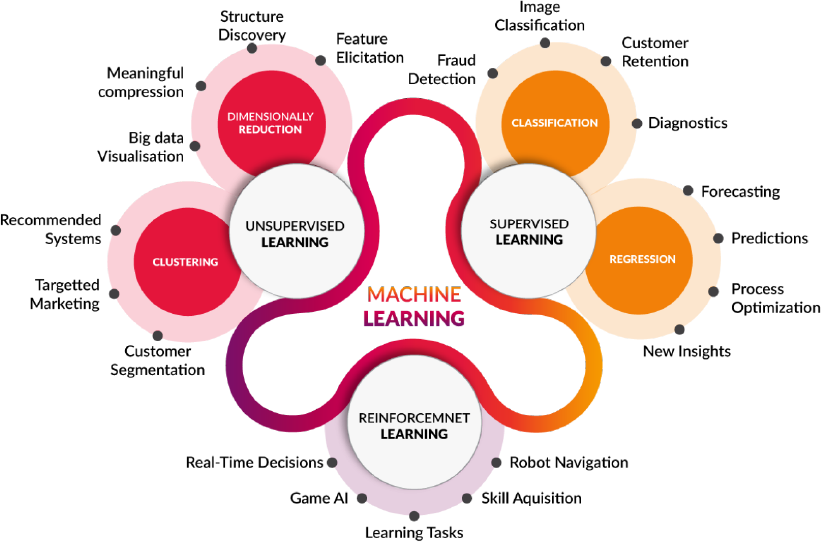
\includegraphics[width=\linewidth]{machine_learning_sections.png}

\subsection{7 Steps of Machine Learning}
\begin{enumerate}
    \item \textcolor{blue}{Gathering data} Collect quantity/quality data for training/testing
    \item \textcolor{blue}{Preparing that data} Cleanup data (remove duplicates, correct errors, deal with missing values, normalize data, convert data types)
    \item \textcolor{blue}{Choosing a model} Select the right algorithm(s)
    \item \textcolor{blue}{Training} Train the model, each iteration of process is a training step
    \item \textcolor{blue}{Evaluation} Use metrics to measure objective performance of the model, test model against previously unseen data, good train/eval split is 80/20, 70/30
    \item \textcolor{blue}{Hyperparameter tuning} Try to improve upon the positive results achieved during the evaluation through gamble with stepNumber of training steps, learning rate, initialization values and distribution
    \item \textcolor{blue}{Prediction} Model should be ready for practical applications
\end{enumerate}

        \section{Natural Language Processing (NLP)}
\begin{itemize}
    \item Automated processing of human language (written \& spoken)
    \item Aims to understand and generate human (natural) language
    \item Understanding spoken text is still difficult
    \item Understanding written text became BIG business (search-engines)
    \item Generating human-like conversations is still very hard
\end{itemize}
\subsection{4 Ingredients of Machine Learning}
\textbf{1. Data}
\begin{itemize}
    \item Dataset
    \item Pre-Processing Pipeline including cleansing, feature-engineering, data augmentation etc.
\end{itemize}
\textbf{2. Cost-Function (Loss)}
\begin{itemize}
    \item Formal mathematical expression for good / bad
    \item Commonly \textcolor{blue}{Mean Squared Error (MSE)}
\end{itemize}
\textbf{3. Model}
\begin{itemize}
    \item From linear model: $\hat{y_i} = ax_i + b$
    \item To complicated million parameter neural networks
    \item Different tasks require different models (regression / decision tree)
\end{itemize}
\textbf{4. Optimization Procedure}
\begin{itemize}
    \item Algorithm that changes the parameters of the model that the cost-function is minimized.
    \item E.g. Stochastic Gradient Descent (SGD), ADAM, RMSProp...
\end{itemize}

For successful ML, there are many more ingredients ...\\
\textbf{5. Performance optimization}
\begin{itemize}
    \item Building of efficient pipelines
    \item Folowwing tool specific recommendations
\end{itemize}
\textbf{6. Visualization and evaluation of the learning Process}
\begin{itemize}
    \item Learning curves
    \item Performance measures
    \item Tensorboard
\end{itemize}
\textbf{7. Cross-Validation \& Regularization}
\begin{itemize}
    \item Train models that generalize well to unseen data
    \item Estimate the generalization error
\end{itemize}

\subsection{Representation of Words}
Vectors can be used to represent words based on their meaning.
\subsubsection{One-hot representation}
\begin{itemize}
    \item Vector with a single 1-Value
    \item All other Values are set to 0
    \item Count the Number of different Words, Define one unique vector per word
\end{itemize}
\textit{Dini Mom isch fett.}\\
Dini: $\begin{bmatrix} 1\\ 0\\ 0\\ 0\\ 0\end{bmatrix}$
Mom: $\begin{bmatrix} 0\\ 1\\ 0\\ 0\\ 0\end{bmatrix}$
isch: $\begin{bmatrix} 0\\ 0\\ 1\\ 0\\ 0\end{bmatrix}$
fett: $\begin{bmatrix} 0\\ 0\\ 0\\ 1\\ 0\end{bmatrix}$
'.': $\begin{bmatrix} 0\\ 0\\ 0\\ 0\\ 1\end{bmatrix}$\\
\textbf{Disadvantages}
\begin{itemize}
    \item Very high dimensional vector space (1 Dimension / unique Word)
    \item Sparse Representation: Each vector has a single 1 and $N$ Zeroes. (Memory Inefficient)
    \item No Generalization: All words are unrelated to each other.
    \item Does not capture any aspect of the meaning of a word
\end{itemize}

\subsubsection{Indexing}
Make a list of words (optionally alphabetically). Use the index to represent each word.\\
\textbf{Example:}\\
\textit{Dini Mom isch fett.}\\
Dini: $0$, Mom: $1$, isch: $2$, fett: $3$, '.': $4$
\begin{itemize}
    \item Dense Equivalent of one-hot encoding
    \item Indexes are not more useful that one-hot vectors
    \item Often used as preprocessing step
    \item Indices / One-Hot Vectors are fed into a network which learns more useful representations
\end{itemize}

\subsubsection{Distributed Representation}
\begin{itemize}
    \item vectors that capture (at least partially) the semantics of a word
    \item Words that occur in similar contexts (neighboring words) tend to have similar meanings
    \item Similar words share similar representations
    \item Distributed representations can be learned
\end{itemize}
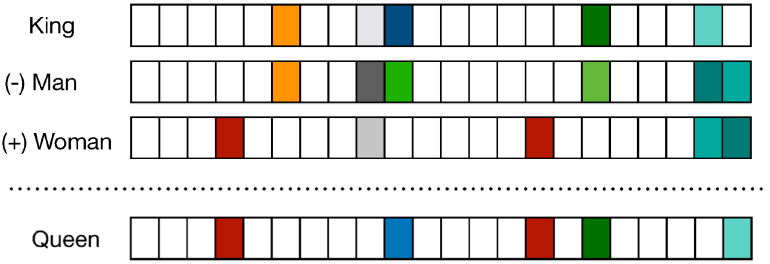
\includegraphics[width=.8\linewidth]{distributed_representation.png}\\
\textbf{Words to Vectors}
\begin{itemize}
    \item Mathematical function maps word to high dimensional Vector
    \item In neural networks, this function is implemented in the Embedding Layer
\end{itemize}
\textbf{Advantage (of vectors)}
\begin{itemize}
    \item Good embedding maps similar/related words to similar regions of the vector space (nearby words have a semantic similarity)
    \item Dot-Product (Skalarprodukt) is a measure of similarity
    \item Possible to add/subtract vectors
\end{itemize}
\textbf{Calculate Similarities between words}
Dot-Product (Skalarprodukt) of 2 Vectors is
\begin{itemize}
    \item maximal when parallel (0\textdegree), both vectors with norm 1 results in max value 1
    \item zero when orthogonal (90\textdegree)
    \item minimal (negative) when opposite directions (180\textdegree) both vectors with norm 1 results in max value -1
\end{itemize}
\textbf{Cosine Distance}
\begin{itemize}
    \item Way to calculate how similar two words (vectors) are
\end{itemize}
cat: A, dog: B \\
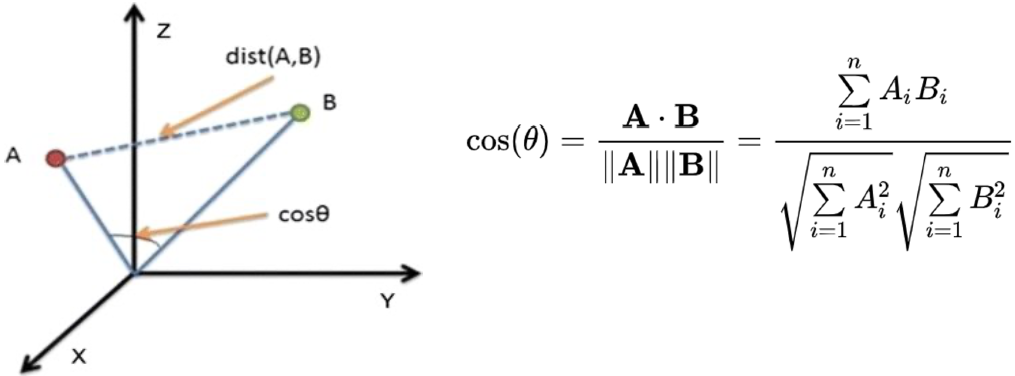
\includegraphics[width=\linewidth]{cosine_distance.png}
Example \\
A: (3, 6, 2, 1), B: (2, 7, 2, 0) \\
$A \cdot B = 6 + 42 + 4 + 0 = 52$ \\
$|| A || || B || = \sqrt{(9 + 36 + 4 + 1)} * \sqrt{(4 + 49 + 4 + 0)} = 53.38539$ \\
$A * B / ( || A || || B ||) = 0.9740$ \\
high value equals high similarity (to be an animal)



        \section{Probability}
\subsection{Random Variables}
\begin{itemize}
    \item Values depend on outcomes of a random phenomenon
    \item Random variable $X$ is a variable that takes a numerical value $x$, which depends on a random experiment
    \item \textcolor{blue}{Discrete} $X$ takes any of a finite set of values ${1.5, 2.123, 6.2, 10}$
    \item \textcolor{blue}{Continous} $X$ takes any value of an uncountable range e.g. real numbers from an interval
\end{itemize}
\textbf{Best we can know}
\begin{itemize}
    \item All possible values
    \item Probability of each value
\end{itemize}
E.g. The discrete random variable $X$ is the number observed when rolling a fair dice.\\
$P(X=x)$ / $P(x)$: $1/6$ for each possible value

\textbf{Joint Probability}
\begin{itemize}
    \item Joint Properties of two random variables
    \item Defined by the Joint Probability Mass Function
\end{itemize}
E.g. Dice1 = 5 AND Dice2 = 4\\
$P_{XY}(5,4) = P_X(5) * P_Y(4) = 1/6 * 1/6 = 1/36$\\
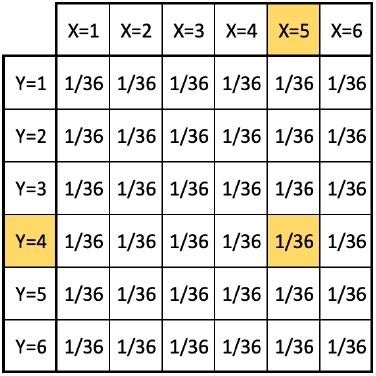
\includegraphics[width=0.5\linewidth]{joint_probability.png} \\
\textbf{Independant random Variables}
\begin{itemize}
    \item Joint Probability is the product of the individual probabilities
\end{itemize}
$P(X,Y) = P(X) * P(Y)$ (only if independant)\\
$P(X,Y,Z) = P(X) * P(Y) * P(Z)$ (only if independant)\\
\textbf{Correlated random Variables}
\begin{itemize}
    \item There are events that are not independant
    \item Such random variables are correlated
    \item $X$: observe clouds (0=no, 1=small, 2=big)
    \item $Y$: observe rain (0=no, 1=light, 2=moderate, 3=heavy)
\end{itemize}
\textbf{Conditional Probability}
\begin{itemize}
    \item One variable is no longer random
    \item X is observed, its value is fixed
    \item Calculate the probabilities of Y given X: $P(Y | X)$
\end{itemize}
$P(X, Y) = P(X | Y) * P(Y)$\\
$P(X, Y) = P(Y | X) * P(X)$\\
$P(Y | X) = \frac{P(X,Y)}{P(X)}$\\
\textbf{Bayes Rule}\\
$P(X|Y)*P(Y) = P(Y|X)*P(X)$\\
Therefore\\
$P(Y|X) = \frac{P(X|Y)*P(Y)}{P(X)}$


\subsection{Probability mass function (PMF)}
Wahrscheinlichkeitsfunktion, a function f(x) that provides the probability for each value x of a discrete random
variable $X$ \\

Graph of a PMF \\
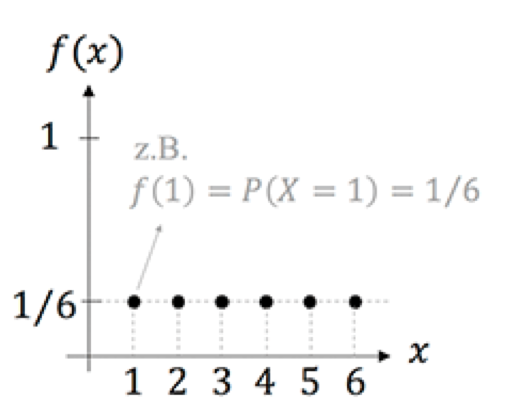
\includegraphics[width=0.2\linewidth]{pmf-graph.png} \\

        \section{Python}

        \section{Data Visualization}
\begin{itemize}
    \item See trends, clusters and local patterns in data
    \item Difficult to see in raw data
    \item Detect outliers and unusual groups
    \item Validate Hypothesis/Conjecture/Theory
\end{itemize}
\vspace{10pt}
\textbf{Important in a Plot}
\begin{itemize}
    \item \textcolor{blue}{X-Axis labels} which data is represented and its units
    \item \textcolor{blue}{Y-Axis labels} which data is represented and its labels
    \item \textcolor{blue}{Title}
    \item \textcolor{blue}{Scale} linear, logarithmic
    \item \textcolor{blue}{Dimensionality of the data 2D / 3D}
\end{itemize}
\vspace{10pt}
\textbf{Dataframe}

a two-dimensional labelled data structure with columns of different types

\subsubsection{Data Analysis Libraries}
\textbf{NumPy}
\begin{itemize}
    \item Package for scientific computing in Python
    \item Multidimensional array object
    \item Routines for fast array operations (sorting, selecting, FFT, linear, ...)
\end{itemize}

\textbf{pandas}
\begin{itemize}
    \item Built on top of NumPy
    \item Routines for accessing tabular data from files (.csv, xls, etc.)
    \item Supports 2-dimensional data (dataframe and series)
    \item Dataframes are something like database tables
\end{itemize}

\textbf{MatPlotLib}
\begin{itemize}
    \item Library for visualizing data
    \item Provides bargraphs, histograms, piecharts, scatter plots, lines, boxplots, heatmaps, ...
\end{itemize}

\textbf{Seaborn}
\begin{itemize}
    \item Extension of MatPlotLib, NumPy and pandas
    \item More user friendly
    \item Plots are aesthetically better
\end{itemize}

\subsubsection{Line Plots}
\begin{itemize}
    \item Bivariate, Continuous
    \item Recognizes trend (pattern of change) (over time)
    \item E.g. Preisgestaltung für Aktienoptionen, Preis von Handys, Bevölkerung eines Lande
\end{itemize}
\subsubsection{Bar Chart}
\begin{itemize}
    \item Used for categorical data
    \item Counting based on each category
    \item E.g. Amount of apps in category Google Play, Apple Store ...
\end{itemize}
\subsubsection{Histogram}
\begin{itemize}
    \item Represents the empirical distribution of a variable
    \item Automatically creates bins (interval) along the range of values
    \item Shows vertical bars to indicate the number of observations per bin
\end{itemize}
\subsubsection{Box Plot (Descriptive Statistics)}

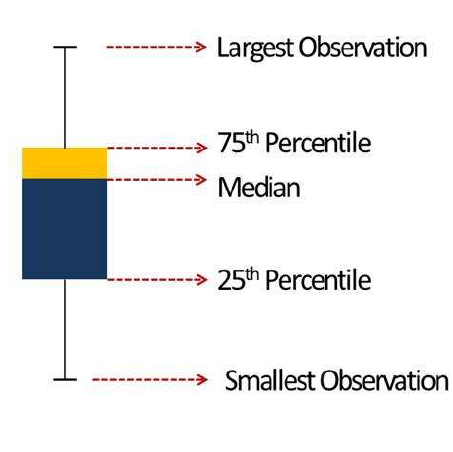
\includegraphics[width=0.5\linewidth]{descriptive_statistics-bx.png}

\textbf{Quartile}

\begin{center}
    $n \cdot p$ ganzzahlig

    $x_p = \frac{1}{2} ( x_{[np]} + x_{[np + 1]})$

    $n \cdot p$ nicht ganzzahlig ($|np|$ auf Ganzzahl abrunden)

    $x_p = x_{[|np|+1]}$ \\
\end{center}

\textcolor{blue}{Quartile 1 (Q1) - 25th Percentile}

$p = 0.25$

25\% der Daten sind kleiner oder gleich diesem Wert. \\

\textcolor{blue}{Quartile 2 (Q2) - 50th Percentile (Median)}

$p = 0.5$

50 \% der Daten sind kleiner oder gleich diesem Wert. Merkmalswert, dessen Merkmalsträger in der Rangordnung aller Merkmalsträger genau die mittlere Position einnimmt. \\

\textcolor{blue}{Quartile 3 (Q3)- 75th Percentile}

$p = 0.75$

75 \% der Daten sind kleiner oder gleich diesem Wert.


\subsubsection{Violin Plots (Descriptive Statistics)}

Wird oftmals verwendet, wenn mehrere Verteilungen von Daten dargestellt werden sollen

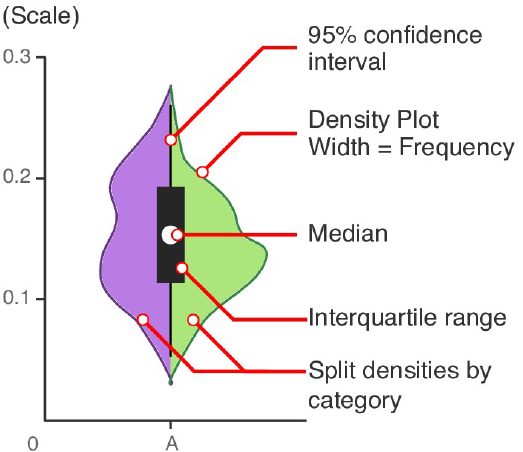
\includegraphics[width=0.5\linewidth]{descriptive_statistics-vio.png}


\subsubsection{Scatter Plot}

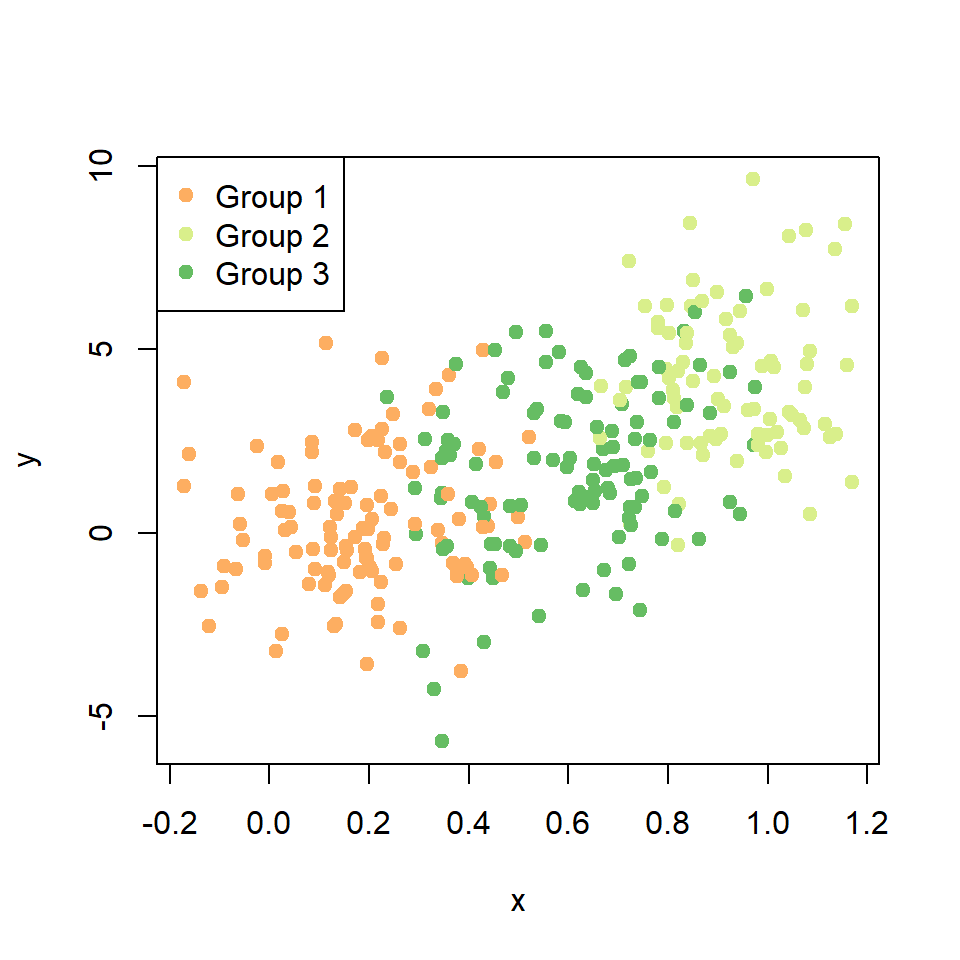
\includegraphics[width=0.7\linewidth]{scatter-plot.png}

\begin{itemize}
    \item Relationship between (two) continuous variables
    \item Helps to get an idea of the degree of correlation between variables
    \item Oftmals nicht hilfreich, wenn Data nichtnumerisch / kategorisch $\rightarrow$ Besser ist in diesem Fall Heat Map
\end{itemize}

        \section{Regression}
\subsection{What is a model?}
In ML, we use the term \textbf{model} for any mathematical function that explains the data:\\ 
$y_i = f(x_i)$\\ 
$y_i = f(x_i) + \epsilon_i$\\ 
where $\epsilon_i$ is unexplained noise. It is often assumed that $\epsilon_i$ follows a normal distribution.\\ 
Instead of approximating $y_i$, we calculate an \textbf{estimate} $\hat{y_i}$ (y hat) of the usually unknown $y_i$: \\
\begin{center}
    $\hat{y_i} = f(x)$
\end{center}

\subsubsection{Linear Regression}
\begin{itemize}
    \item Only consideres a linear relationship between input and output
    \item In the simplest case, $x$ and $y$ are scalars and the linear model therefore has only two free parameters
    \item The goal is to identify $a$ (slope) and $b$ (intercept) for which the linear model best explains the data
\end{itemize}
\begin{center}
    $\hat{y_i} = ax_i + b$
\end{center}

\subsubsection{Mean Squared Error (MSE)}
\begin{itemize}
    \item Loss we want to minimize
    \item Usually divided by 2
\end{itemize}
\begin{center}
    $\hat{y_i} = ax_i + b$\\ 
    $e_i = y_i - \hat{y_i}$ \\ 
    The difference $e_i$, called residual\\ 
    $E = \frac{1}{2N} * \displaystyle\sum_{i = 1}^{N} e_i^2$\\
    $E = \frac{1}{2N} * \large\displaystyle\sum_{i = 1}^{N}(\hat{y_i} - (a*x_i + b))^2$
\end{center}

\subsubsection{Correlation and Causality}
\begin{itemize}
    \item Correlation is not causality
    \item Correlation refers to the degree to which a pair of variables are linearly related
    \item Linear regression is a tool to detect correlations between two or more variables
    \item Correlation can be quantified using the Pearson correlation coefficient
\end{itemize}

    \end{multicols*}
\end{document}

























